\section{The Chainsewing Attack}\label{sec:attack}
We now describe an explicit attack against the NIPoPoW suffix proof construction under velvet fork. As already argued, since the protocol is implemented under velvet fork, any thorny block will be accepted as valid. Taking advantage of such blocks in the chain, the adversary can produce suffix proofs containing an arbitrary number of blocks belonging to several fork chains. The attack works as follows.

Assume chain $\chain_B$ was adopted by an honest party $B$ and chain $\chain_\mathcal{A}$, a fork of $\chain_B$ at some point, is maintained by the adversary $\mathcal{A}$. After the fork point $b = (\chain_B \cap \chain_\mathcal{A})[-1]$, the honest party produces a block extending $b$ in $\chain_B$ containing a transaction $\tx$. The adversary includes a conflicting (double spending) transaction $\tx'$ in a block extending $b$ in $\chain_\mathcal{A}$.
The adversary wants to produce a suffix proof convincing a light client that $\chain_\mathcal{A}$ is the longer chain. In order to achieve this, the adversary needs to include a greater amount of total proof-of-work in her suffix proof, $\pi_\mathcal{A}$, in comparison to that included in the honest party's proof, $\pi_B$, so as to achieve $\pi_\mathcal{A} \geq_m \pi_B$. Towards this purpose, she miners intermittently on both $\chain_B$ and $\chain_\mathcal{A}$. She produces some thorny blocks in both chains $\chain_\mathcal{A}$ and $\chain_B$ which will allow her to usurp selected blocks of $\chain_B$ and present them to the light client as if they belonged to $\chain_\mathcal{A}$ in her suffix proof.

The general form of this attack for an adversary sewing blocks to one forked chain is illustrated in Figure~\ref{fig:generic_attack}. Dashed arrows represent interlink pointers of some level $\mu_\mathcal{A}$. Starting from a thorny block in the adversary's forked chain and following the interlink pointers, jumping between $\chain_\mathcal{A}$ and $\chain_B$, a chain of blocks crossing forks is formed, which the adversary claims as part of her suffix proof. Blocks of both chains are included in this proof and a verifier cannot distinguish the non-smooth pointers participating in this proof chain and, as a result, considers it a valid proof.

\begin{figure}[h]
	\begin{center}
		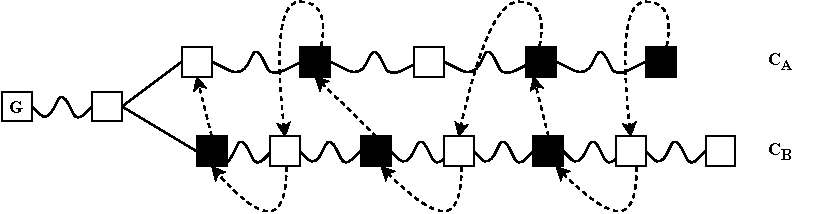
\includegraphics[width=0.95\columnwidth
		]{figures/generic_chainsewing_attack.pdf}
	\end{center}
	\caption{Generic Chainsewing Attack. $\chain_B$ is the chain of an honest party and $\chain_\mathcal{A}$ the adversary's chain. Adversarially generated blocks are 	colored black. Dashed arrows represent interlink pointers included in the	adversary's suffix proof. Wavy lines imply one or more blocks.}
	\label{fig:generic_attack}
\end{figure}

This generic attack can be made concrete as follows.
The adversary chooses to attack at some level $\mu_\mathcal{A} \in \mathbb{N}$. As shown in Figure~\ref{fig:attack}, she first generates a superblock $b'$ in her forked chain $\chain_\mathcal{A}$ and a thorny block $a'$ in the honest chain $\chain_B$ which points to $b'$. Block $a'$ will be accepted as valid in the honest chain $\chain_B$ despite the invalid interlink pointers. Subsequently, the adversary waits for a period of time until the honest parties have produced a certain number of $\mu_\mathcal{A}$-superblocks in $\chain_B$.
Let $b$ denote the last such honestly generated $\mu_\mathcal{A}$-superblock.
She then attempts to mine a thorny block $a$ in $\chain_\mathcal{A}$ pointing to $b$ of $\chain_B$. Because of the way blocks are generated by upgraded honest miners, there will be successive interlink pointers leading from block $b$ to block $a'$. Thus following the interlink pointers a chain is formed which connects $\chain_\mathcal{A}$ blocks $a$ and $b'$ and contains an arbitrarily large part of the honest party's chain $\chain_B$. At this point, the adversary continues mining on top of block $a$.

When the time arrives for the adversary to produce the NIPoPoW, she produces a suffix proof for chain $\chain_\mathcal{A}$ containing the subchain $\chain_\mathcal{A}\{{:}b'\} \conc b' \conc \chain\{a'{:}b\} \conc b \conc \chain_\mathcal{A}\{a{:}\}$. Note that following the interlink pointers constructed in such a way, a light client perceives this $\mu_\mathcal{A}$-superchain as a valid chain, as he cannot detect it is spanning across different forks at level $0$.

\begin{figure}[h!]
	\begin{center}
		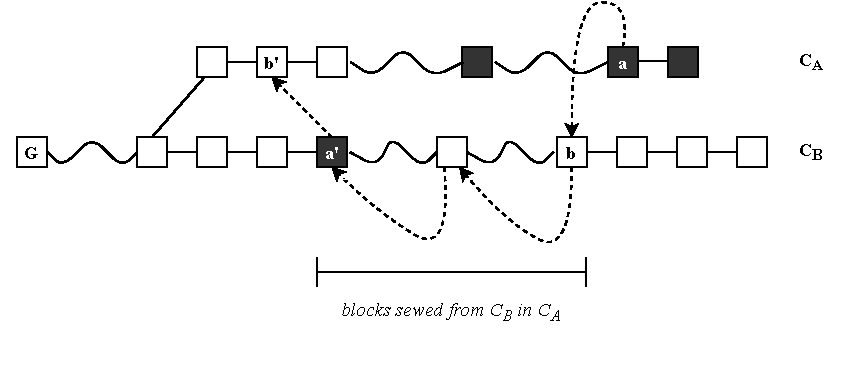
\includegraphics[width=\columnwidth]{figures/chainsewing_attack.pdf}
	\end{center}
	\caption{Chainsewing Attack. $\chain_B$ represents the chain of an honest party. $\chain_\mathcal{A}$ is an adversarial fork. Adversarially generated blocks are colored black. Dashed arrows represent interlink pointers included in the adversary's suffix proof. Wavy lines imply one or more blocks. Firm lines imply the \emph{previd} relationship between two sequential blocks.}
	\label{fig:attack}
\end{figure}

In this attack the adversary uses thorny blocks to ``sew'' portions of the honestly adopted chain to her own forked chain. This remark justifies the name given to the attack.

Note that in order to make this attack successful, the adversary needs only produce few superblocks which let her arrogate an arbitrarily large number of blocks. Thus this attack succeeds with non-negligible probability.
